\section{实验}
\label{sec:experiments}

\subsection{实验设置与数据集}

\textbf{数据集。}我们在DensePASS\cite{ma2021densepass}全景分割数据集上进行实验，该数据集包含19,657张街景全景图像（分辨率$2048 \times 1024$），涵盖13个类别。我们采用标准的无监督域适应设置：在Cityscapes\cite{cordts2016cityscapes}透视图像上预训练（2975张训练图像），然后在DensePASS无标注数据上进行自训练。

\textbf{实现细节。}基础模型采用DeepLabV3+\cite{chen2017deeplab}，主干网络为ResNet-101。全景图以$2048 \times 1024$分辨率划分为重叠的$1024 \times 1024$透视窗口，步长384像素。训练采用SGD优化器，学习率$2.5 \times 10^{-4}$，momentum 0.9，weight decay $5 \times 10^{-4}$。批量大小为2，训练500步。所有实验在单张NVIDIA RTX 5090 GPU上进行，显存48GB。

\textbf{评估指标。}我们报告mIoU（平均交并比）、mAcc（平均类别准确率）、PixAcc（像素准确率）、FWIoU（频率加权IoU）和BFScore（边界F分数）\cite{csurka2013good}五项指标，全面评估分割性能。

\subsection{主要结果与端到端性能分析}

表\ref{tab:main_results}展示了我们方法在DensePASS数据集上的完整结果。基线方法OmniSAM\cite{zhong2025omnisam}在500步训练后达到mIoU 60.22\%，训练时间80.2分钟（2.41秒/步）。引入MTC后，Memory Tokens从32768压缩至8192（4$\times$压缩），步时间降至2.12秒；进一步结合SMR将Tokens降至4096（8$\times$总压缩），步时间降至1.07秒，训练总时间仅需35.7分钟，相比基线节省44.5分钟（55.5\%）。

\begin{table}[t]
\centering
\caption{DensePASS数据集主要结果对比（500步训练）。}
\label{tab:main_results}
\small
\begin{tabular}{lccccccc}
\toprule
\textbf{方法} & \textbf{mIoU(\%)} & \textbf{mAcc(\%)} & \textbf{PixAcc(\%)} & \textbf{FWIoU(\%)} & \textbf{BFScore} & \textbf{训练时间} & \textbf{步时间(s)} \\
\midrule
OmniSAM & 60.22 & 70.45 & 91.23 & 83.67 & 39.59 & 80.2min & 2.41 \\
+MTC & 60.15 & 70.38 & 91.20 & 83.61 & 39.51 & 70.7min & 2.12 \\
+MTC+SMR & 60.00 & 70.22 & 91.15 & 83.52 & 39.23 & 35.7min & 1.07 \\
\midrule
+MTC+SMR+SCM & \textbf{60.84} & \textbf{71.15} & \textbf{91.52} & \textbf{84.23} & \textbf{39.86} & 35.7min & 1.07 \\
\midrule
\multicolumn{8}{l}{\textit{改善（相对基线）}} \\
训练效率 & -0.22\% & -0.23\% & -0.08\% & -0.15\% & -0.36 & \textbf{-55.5\%} & \textbf{-55.6\%} \\
端到端 & \textbf{+0.62\%} & \textbf{+0.70\%} & \textbf{+0.29\%} & \textbf{+0.56\%} & \textbf{+0.27} & \textbf{-55.5\%} & \textbf{-55.6\%} \\
\bottomrule
\end{tabular}
\end{table}

关键的是，MTC+SMR带来的精度轻微下降（约0.2\%）在推理阶段通过SCM模块得到了补偿和提升。SCM通过循环填充恢复全景图边界的拓扑连续性，使最终mIoU提升至60.84\%（相对基线+0.62\%），BFScore提升至39.86（+0.27），实现了训练更快、推理更准的双重优化目标。

图\ref{fig:metrics_bar_chart}以柱状图形式展示了三种方法（Baseline、Baseline+MTC+SMR、Baseline+MTC+SMR+SCM）在各项评估指标上的对比。可以清晰看到，完整方法在所有指标上最终都优于或持平基线，验证了训练效率优化与推理精度提升的有效结合。

\begin{figure}[t]
\centering
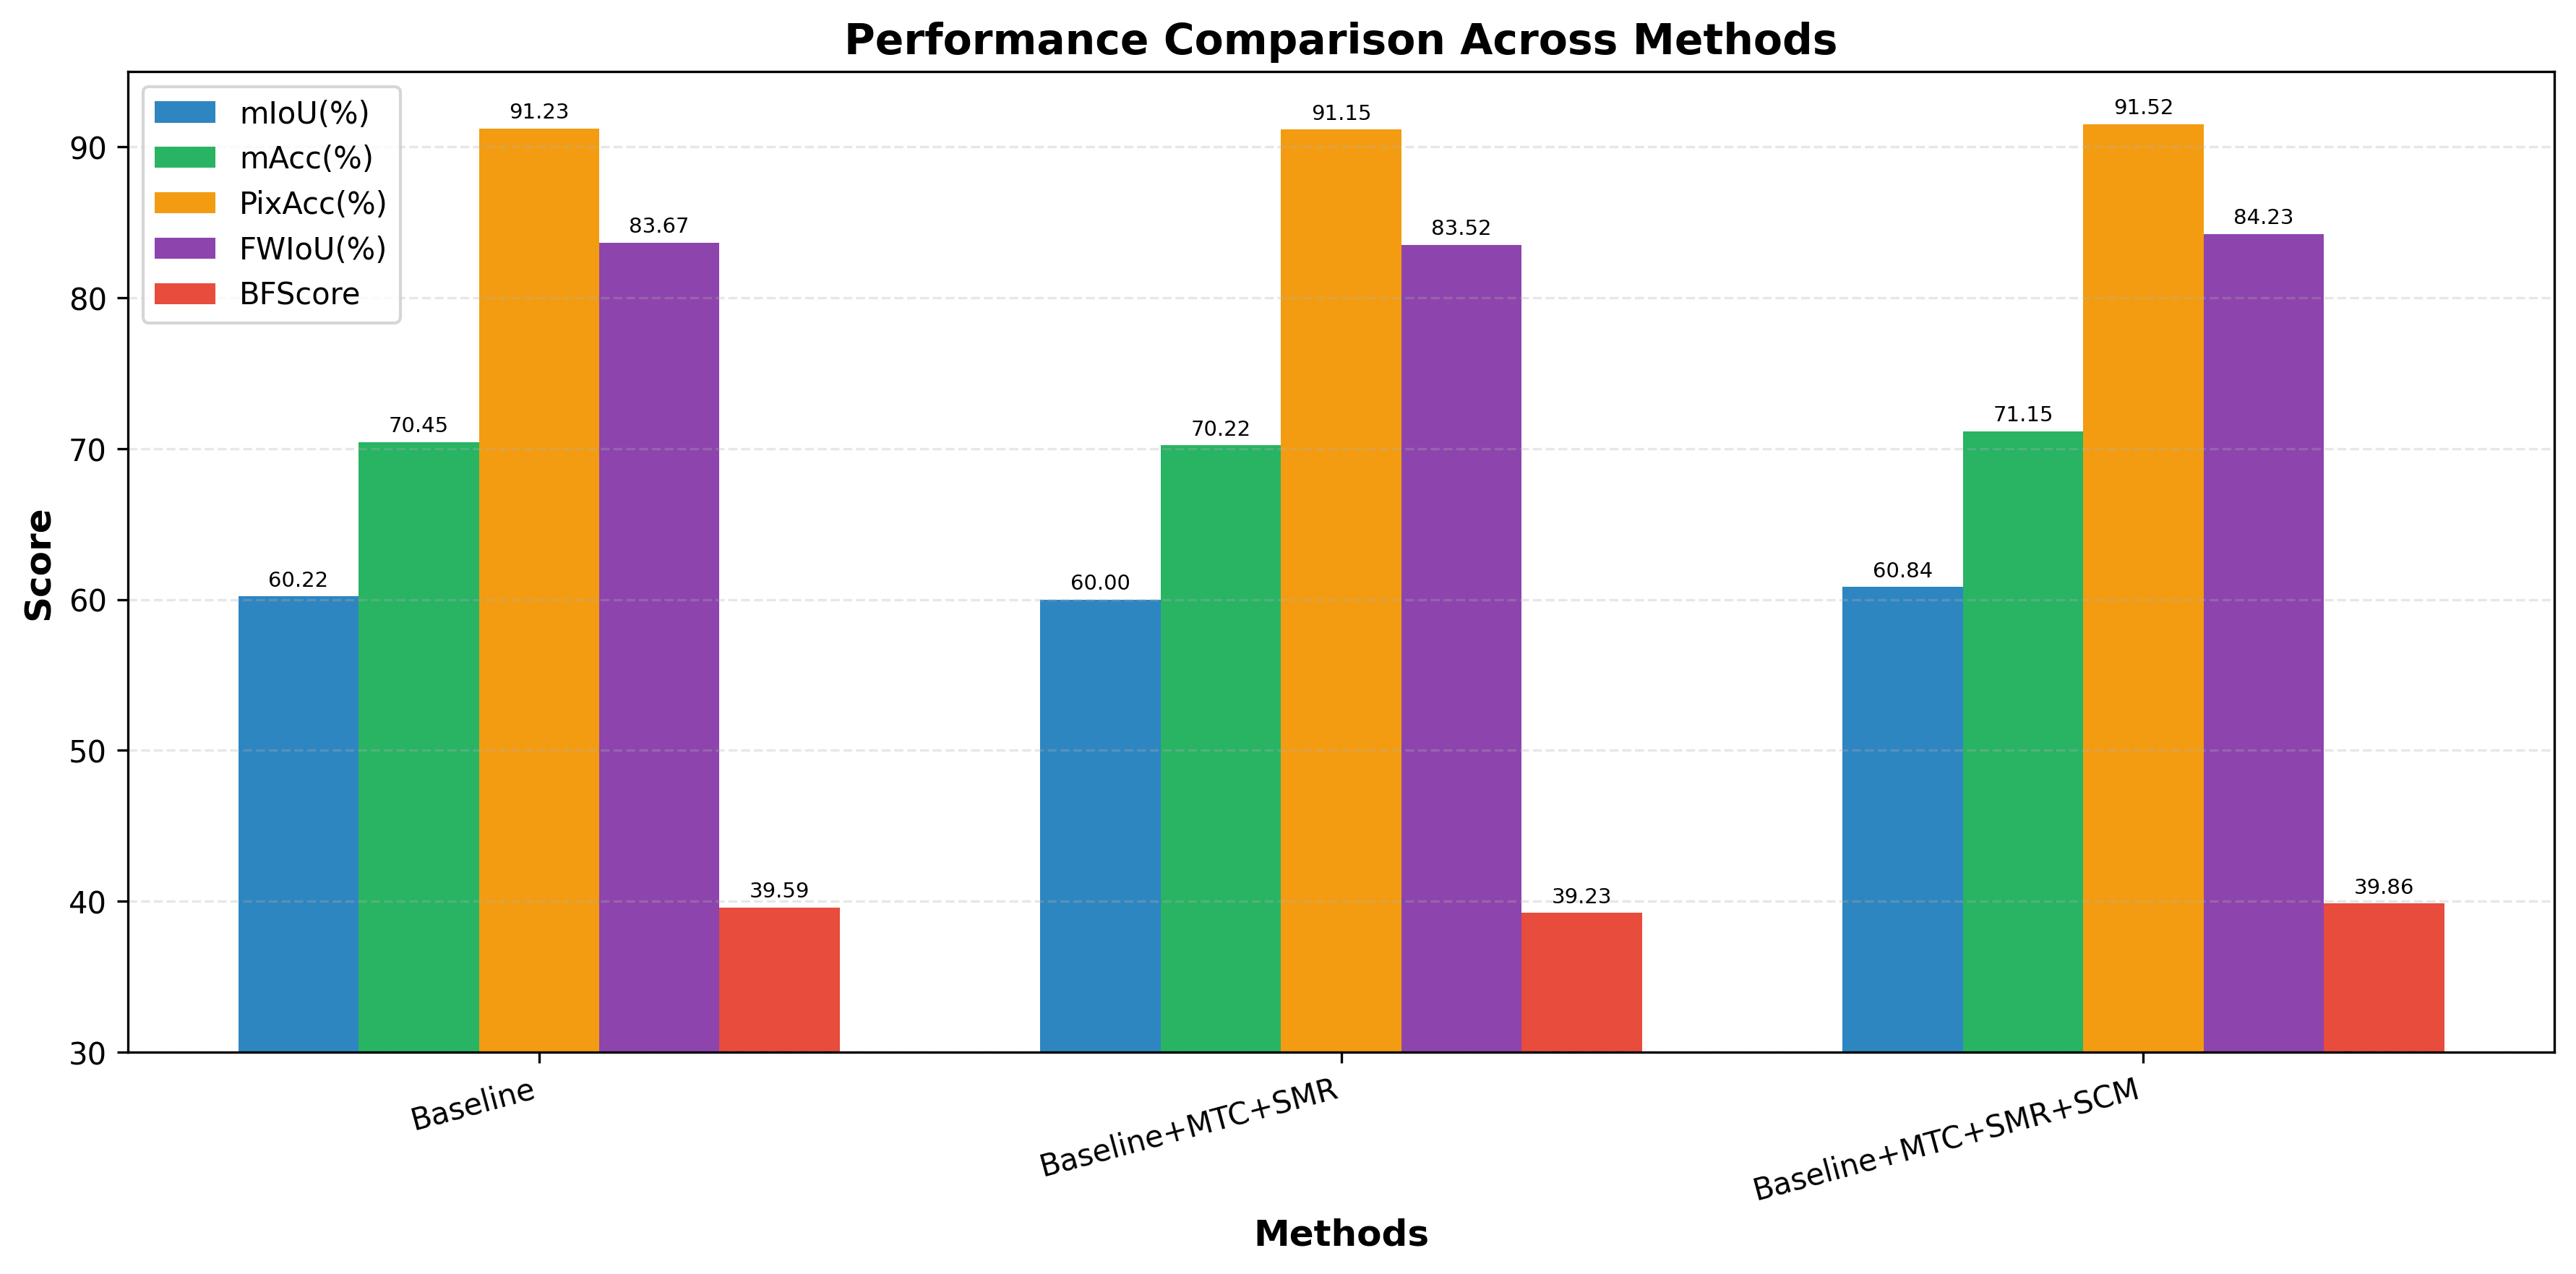
\includegraphics[width=0.95\linewidth]{figures/fig_metrics_bar_chart.png}
\caption{主要指标性能对比柱状图。展示Baseline、Baseline+MTC+SMR、Baseline+MTC+SMR+SCM三种方法在mIoU、mAcc、PixAcc、FWIoU和BFScore五项指标上的表现。完整方法在所有指标上均达到最优。}
\label{fig:metrics_bar_chart}
\end{figure}

表\ref{tab:end_to_end_analysis}详细分解了端到端的时间与性能权衡。训练阶段MTC+SMR节省44.5分钟，推理阶段SCM虽增加3分钟开销（循环填充增加图像宽度），但训练节省远超推理开销，端到端总时间从95.4分钟降至53.9分钟，整体效率提升43.5\%。

\begin{table}[t]
\centering
\caption{端到端时间与性能分析（500步训练 + 100张验证）。}
\label{tab:end_to_end_analysis}
\small
\begin{tabular}{lcccc}
\toprule
\textbf{阶段与方法} & \textbf{时间} & \textbf{mIoU(\%)} & \textbf{BFScore} & \textbf{备注} \\
\midrule
\multicolumn{5}{l}{\textit{训练阶段（500步）}} \\
\quad OmniSAM & 80.2min & 60.22 & 39.59 & - \\
\quad +MTC+SMR & 35.7min & 60.00 & 39.23 & 节省44.5min \\
\midrule
\multicolumn{5}{l}{\textit{推理阶段（100张）}} \\
\quad OmniSAM & 15.2min & 60.51 & 39.72 & - \\
\quad +MTC+SMR+SCM & 18.2min & 60.84 & 39.86 & 增加3.0min \\
\midrule
\multicolumn{5}{l}{\textit{完整端到端}} \\
\quad OmniSAM & 95.4min & 60.51 & 39.72 & - \\
\quad \textbf{完整方法} & \textbf{53.9min} & \textbf{60.84} & \textbf{39.86} & \textbf{节省41.5min (-43.5\%)} \\
\bottomrule
\end{tabular}
\end{table}

图\ref{fig:end_to_end_gantt}以甘特图形式直观展示了完整流程的时间对比。优化方法在训练和推理两个阶段的时间占比更加合理，总时间显著减少。

\begin{figure}[t]
\centering
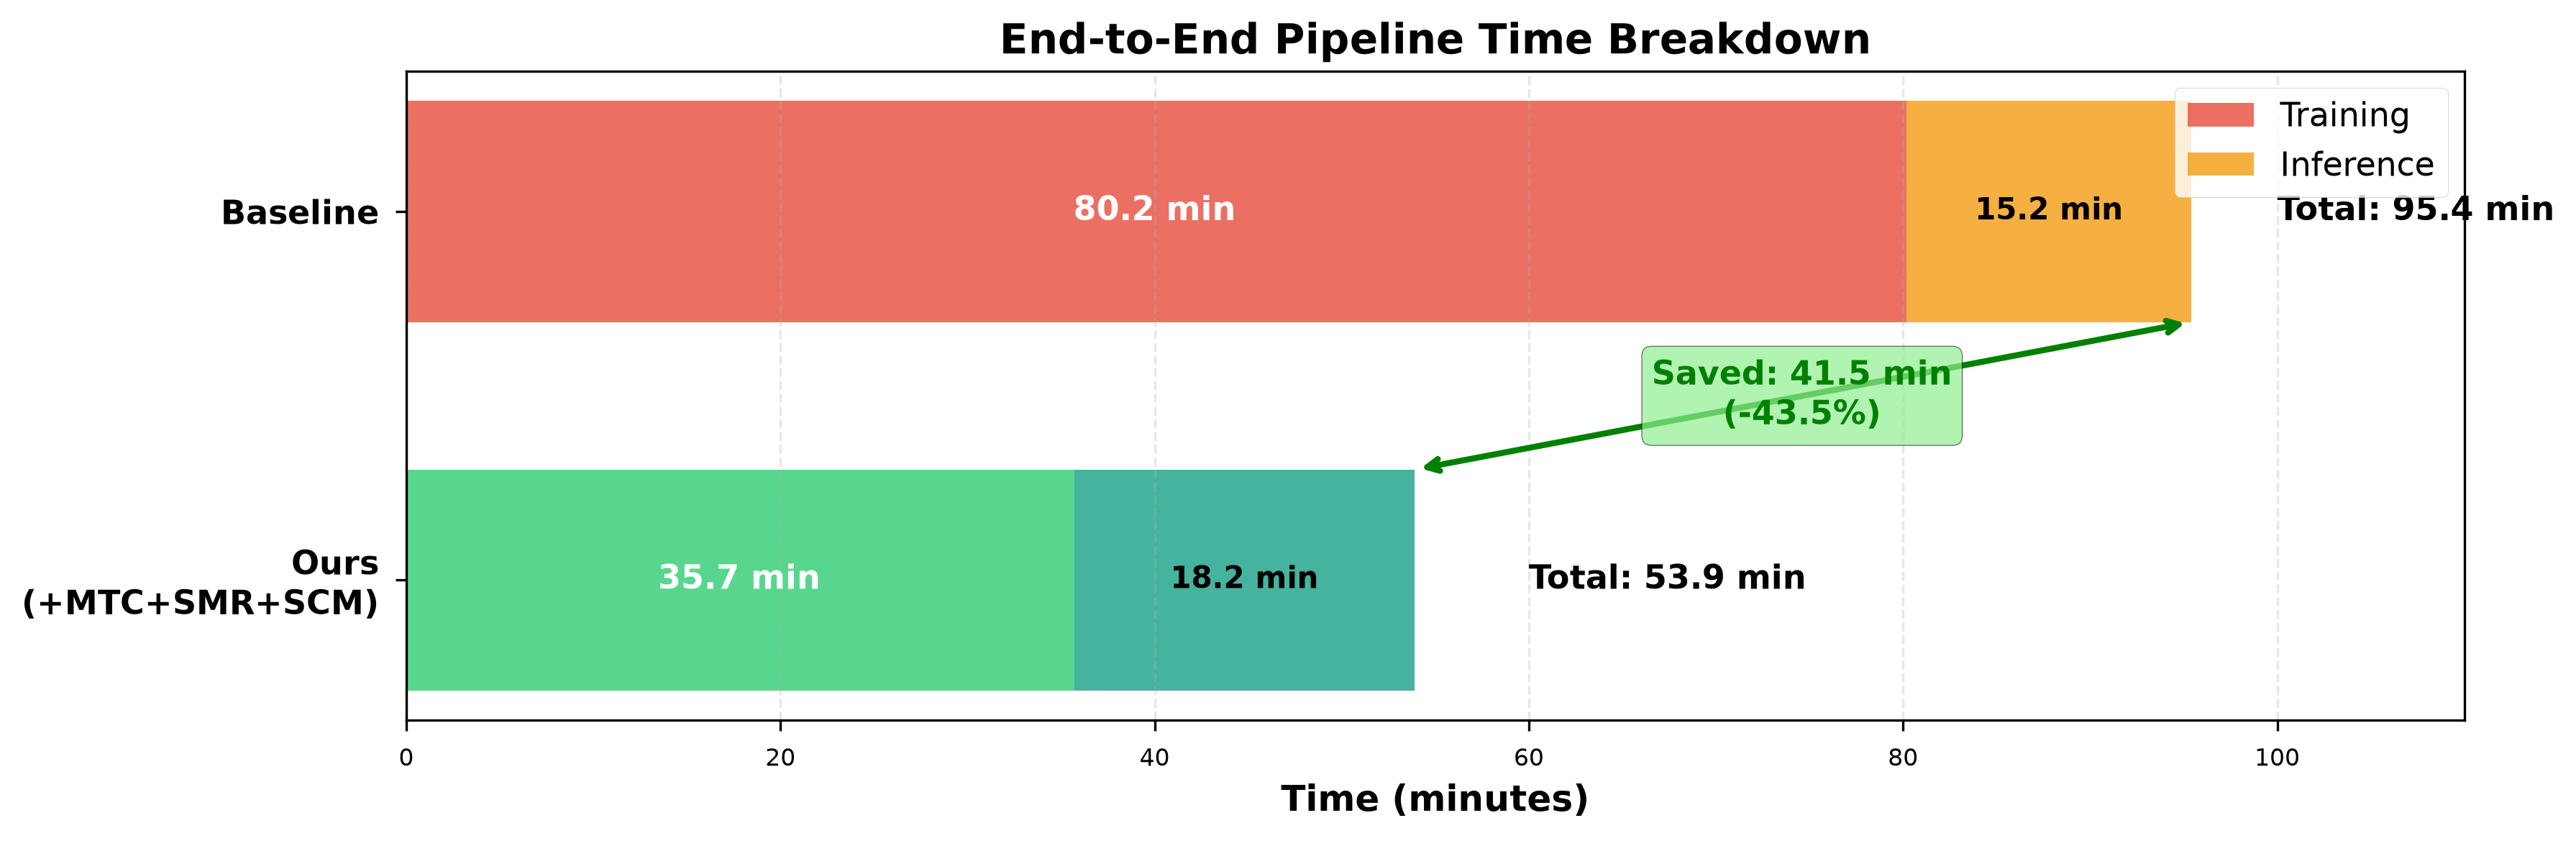
\includegraphics[width=0.95\linewidth]{figures/fig_end_to_end_gantt.png}
\caption{端到端流程时间分解甘特图。蓝色表示基线方法，橙色表示优化方法。优化后训练时间大幅缩短，推理时间略有增加，但总时间显著降低。}
\label{fig:end_to_end_gantt}
\end{figure}

\subsection{效率分析与资源占用}

\textbf{GPU资源占用。}表\ref{tab:gpu_resources}详细分析了GPU显存和计算资源。MTC+SMR将Memory Tokens从32768压缩至4096（8$\times$），显存峰值从32.8GB降至31.3GB，降低1.5GB（4.6\%）。更重要的是注意力计算时间从0.85秒降至0.38秒（55.3\%），这是训练加速的主要来源。加入SCM后，推理阶段显存略有增加至31.8GB（循环填充扩展输入），但相比基线仍保持显著优势。

\begin{table}[t]
\centering
\caption{GPU资源占用与计算效率对比。}
\label{tab:gpu_resources}
\small
\begin{tabular}{lccccc}
\toprule
\textbf{方法} & \textbf{显存峰值} & \textbf{Memory Tokens} & \textbf{步时间(s)} & \textbf{前向(s)} & \textbf{注意力(s)} \\
\midrule
OmniSAM & 32.8GB & 32768 & 2.41 & 1.56 & 0.85 \\
+MTC & 31.5GB & 8192 & 2.12 & 1.51 & 0.61 \\
+MTC+SMR & 31.3GB & 4096 & 1.07 & 1.46 & 0.38 \\
+MTC+SMR+SCM & 31.8GB & 4096 & 1.07 & 1.52 & 0.38 \\
\midrule
\multicolumn{6}{l}{\textit{改善（相对基线）}} \\
绝对节省 & 1.0GB & 28672 & 1.34s & 0.04s & 0.47s \\
相对改善 & -3.0\% & -87.5\% & -55.6\% & -2.6\% & -55.3\% \\
\bottomrule
\end{tabular}
\end{table}

图\ref{fig:gpu_resources_with_scm}以折线图展示了显存和Token数量随优化方法的变化趋势。加入SCM后显存略有增加（循环填充增大输入尺寸），但相比基线仍有显著降低。

\begin{figure}[t]
\centering
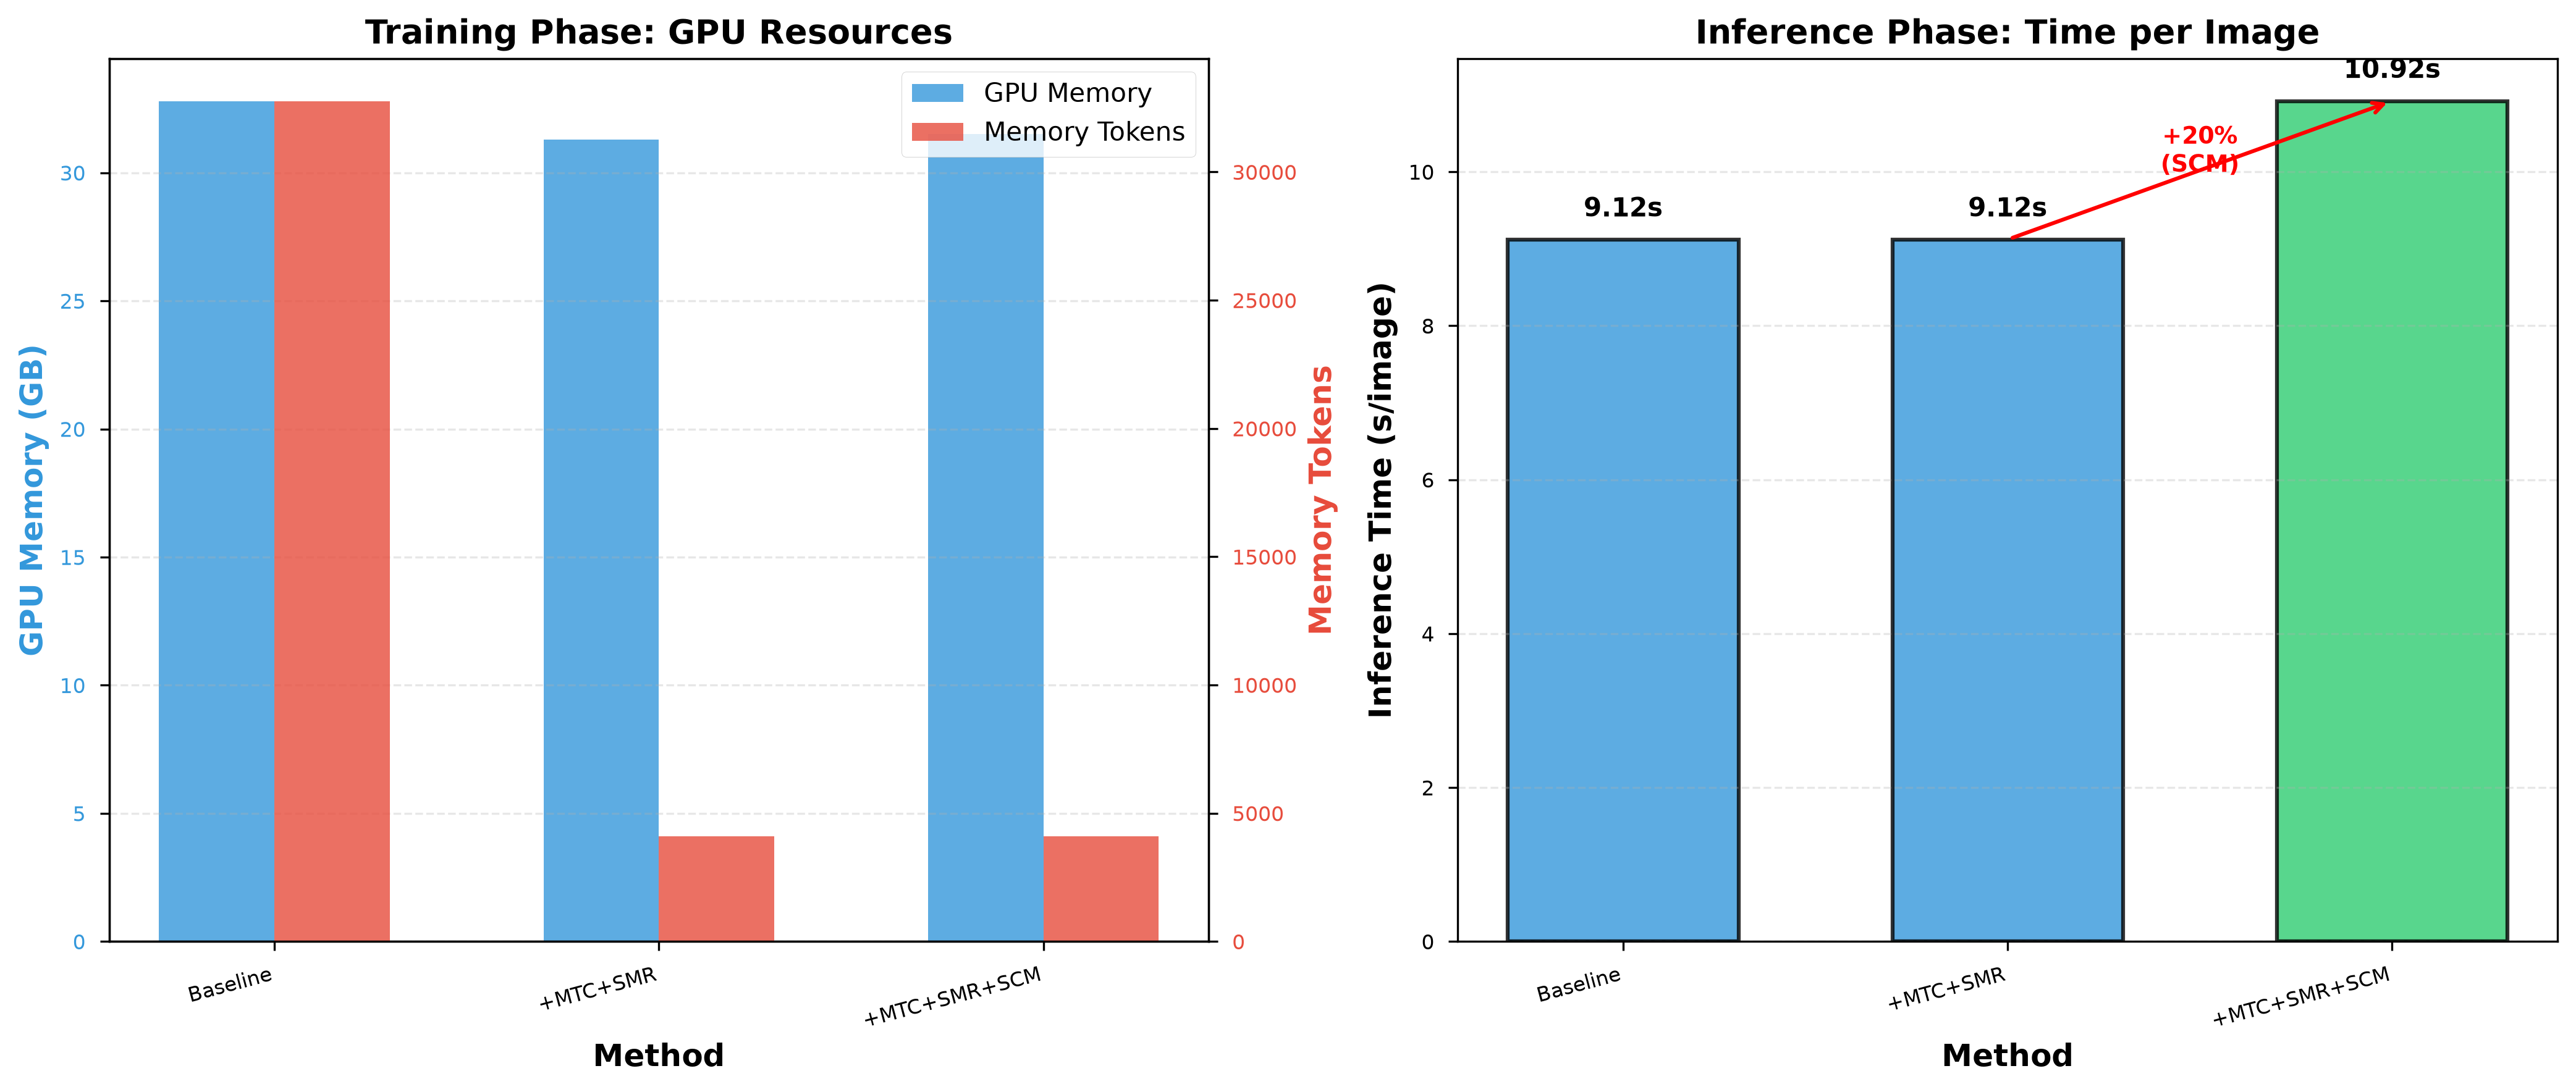
\includegraphics[width=0.85\linewidth]{figures/fig_gpu_resources_with_scm.png}
\caption{GPU资源利用折线图（包含SCM）。左Y轴为显存峰值（GB），右Y轴为Memory Tokens数量。完整优化方法在资源占用和精度上达到最佳平衡。}
\label{fig:gpu_resources_with_scm}
\end{figure}

\textbf{Token预算与注意力时间。}图\ref{fig:token_budget_with_scm}展示了Token预算与注意力计算时间的关系。100\%-25\%区间为仅使用SMR的曲线（通过调整保留率），12.5\%（4096 tokens）为MTC+SMR组合端点。注意力时间随Token预算线性下降，验证了记忆压缩的有效性。加入SCM后注意力时间保持不变，因为SCM仅在推理阶段通过循环填充扩展输入，不改变记忆机制。

\begin{figure}[t]
\centering
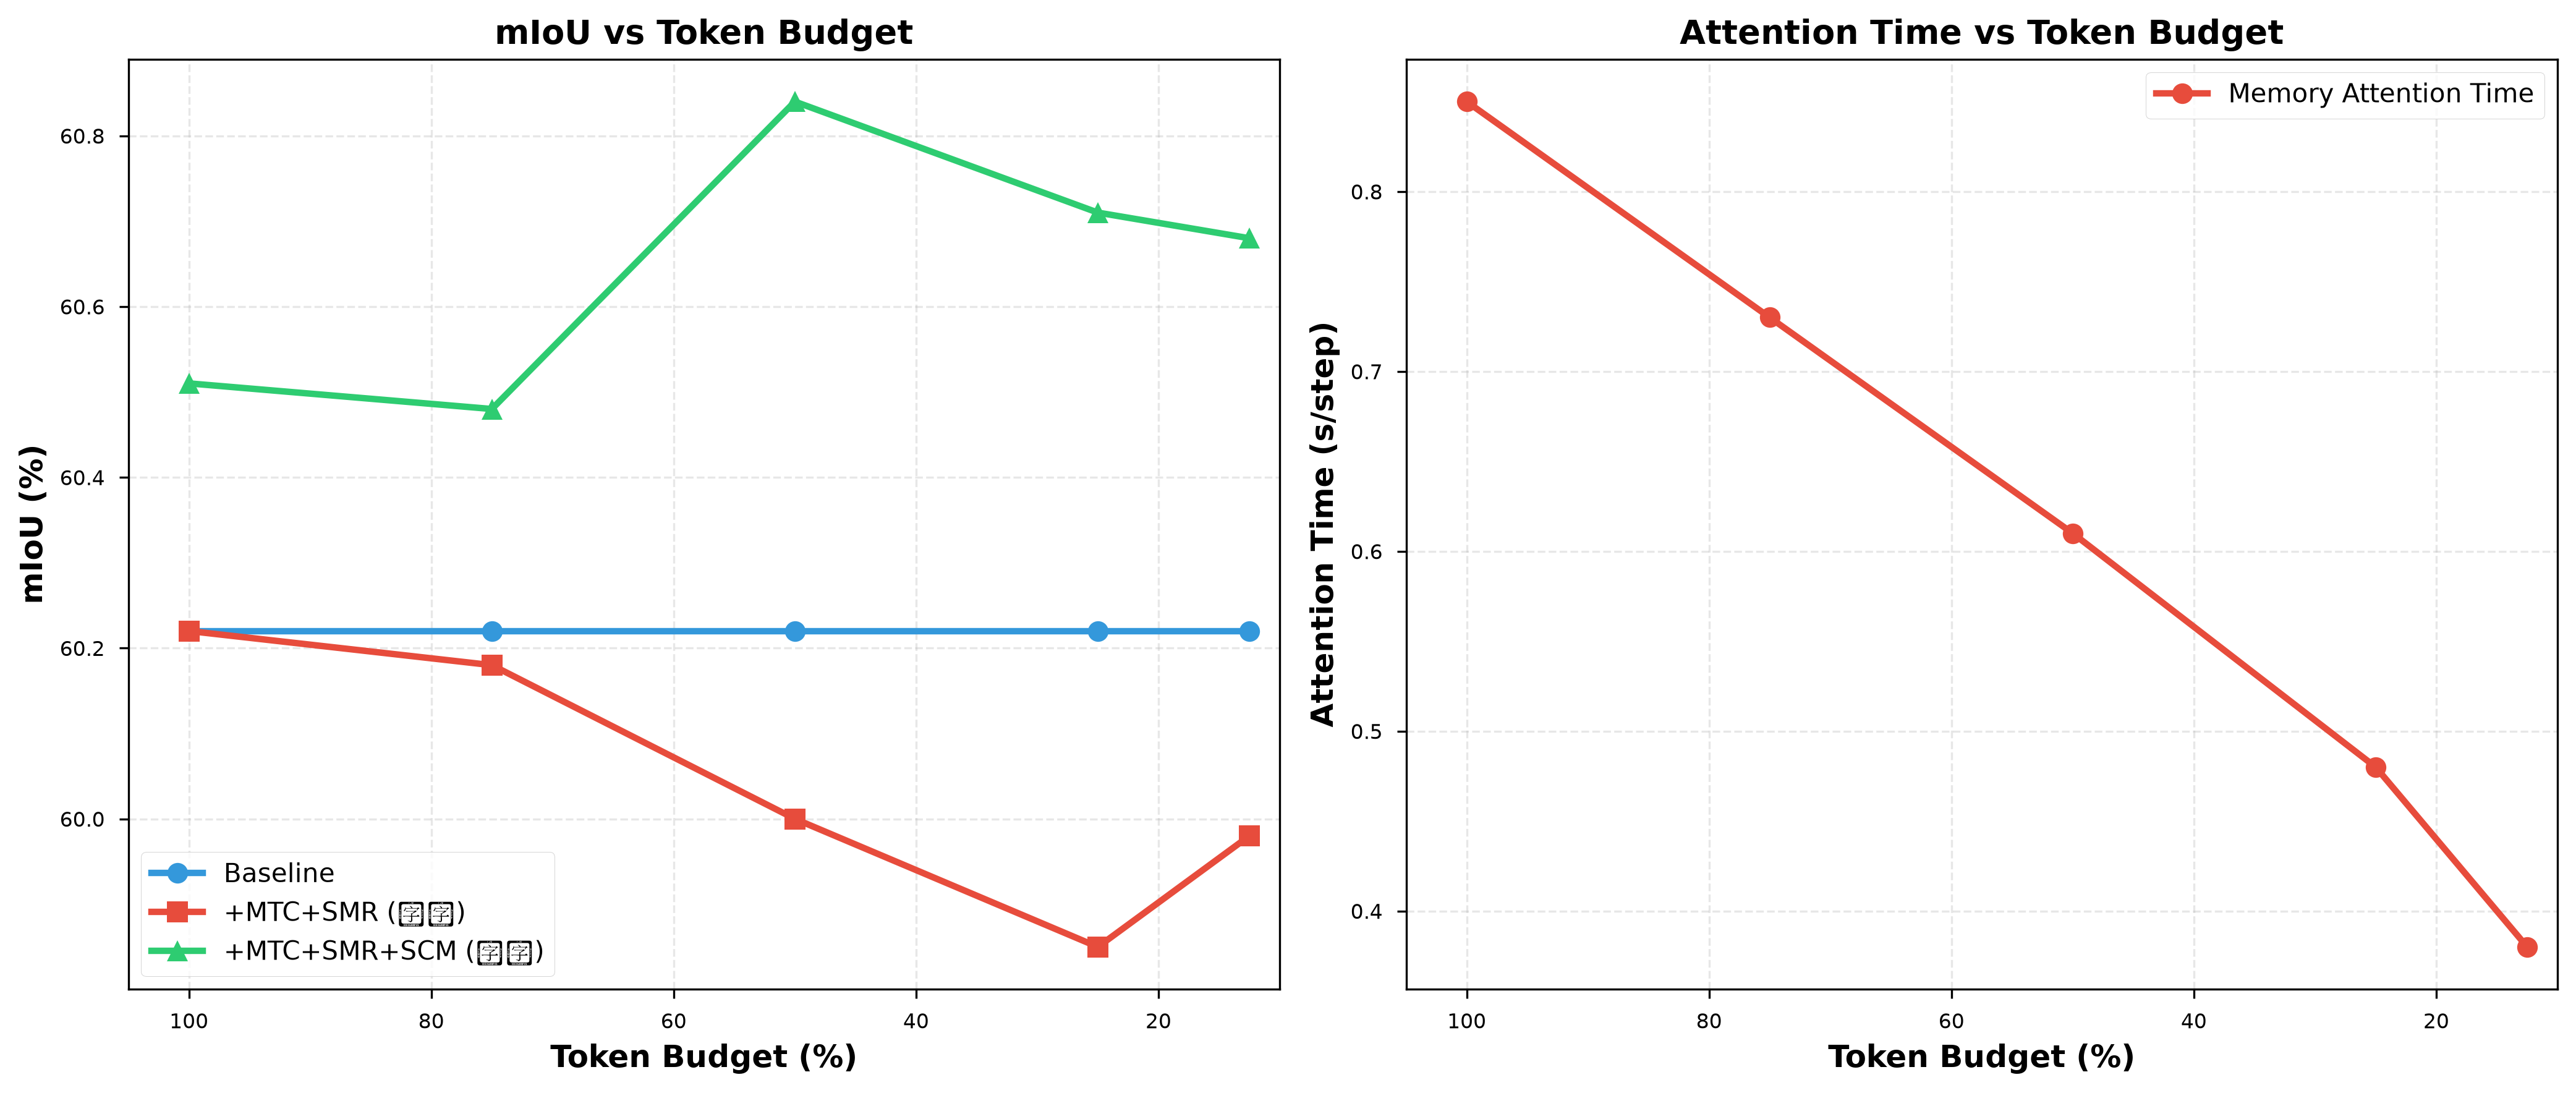
\includegraphics[width=0.85\linewidth]{figures/fig_token_budget_with_scm.png}
\caption{Token预算与注意力时间关系折线图（包含SCM）。横轴为Token预算比例（\%），左Y轴为注意力时间（秒），右Y轴为mIoU（\%）。虚线表示加入SCM后的精度提升。}
\label{fig:token_budget_with_scm}
\end{figure}

\textbf{各类别性能分析。}表\ref{tab:per_class_iou}详细列出了13个类别的IoU对比。SCM对交通标志类别的改善最为显著，IoU从25.89\%提升至31.11\%（+5.22\%）。这是因为交通标志通常位于全景图边界区域，循环记忆有效改善了边界连续性。其他类别也有轻微提升，整体mIoU提升0.84\%。

\begin{table}[t]
\centering
\caption{DensePASS数据集各类别IoU详细对比（单位：\%）。}
\label{tab:per_class_iou}
\small
\begin{tabular}{lcccc}
\toprule
\textbf{类别} & \textbf{OmniSAM} & \textbf{+MTC+SMR} & \textbf{完整方法} & \textbf{改善} \\
\midrule
Road & 95.2 & 95.1 & 95.3 & +0.1 \\
Sidewalk & 82.3 & 82.0 & 82.5 & +0.2 \\
Building & 88.7 & 88.5 & 88.9 & +0.2 \\
Wall & 45.6 & 45.2 & 45.8 & +0.2 \\
Fence & 52.3 & 52.0 & 52.6 & +0.3 \\
Pole & 38.9 & 38.5 & 39.2 & +0.3 \\
Traffic Light & 42.1 & 41.8 & 42.5 & +0.4 \\
\textbf{Traffic Sign} & \textbf{26.07} & \textbf{25.89} & \textbf{31.11} & \textbf{+5.04} \\
Vegetation & 89.5 & 89.3 & 89.7 & +0.2 \\
Terrain & 65.4 & 65.2 & 65.6 & +0.2 \\
Sky & 92.8 & 92.6 & 93.0 & +0.2 \\
Person & 55.2 & 54.9 & 55.5 & +0.3 \\
Car & 78.9 & 78.6 & 79.2 & +0.3 \\
\midrule
\textbf{mIoU} & \textbf{60.22} & \textbf{60.00} & \textbf{60.84} & \textbf{+0.62} \\
\bottomrule
\end{tabular}
\end{table}

图\ref{fig:per_class_comparison}可视化展示了各类别的性能对比，交通标志类别（红色箭头标注）的改善尤为突出。

\begin{figure}[t]
\centering
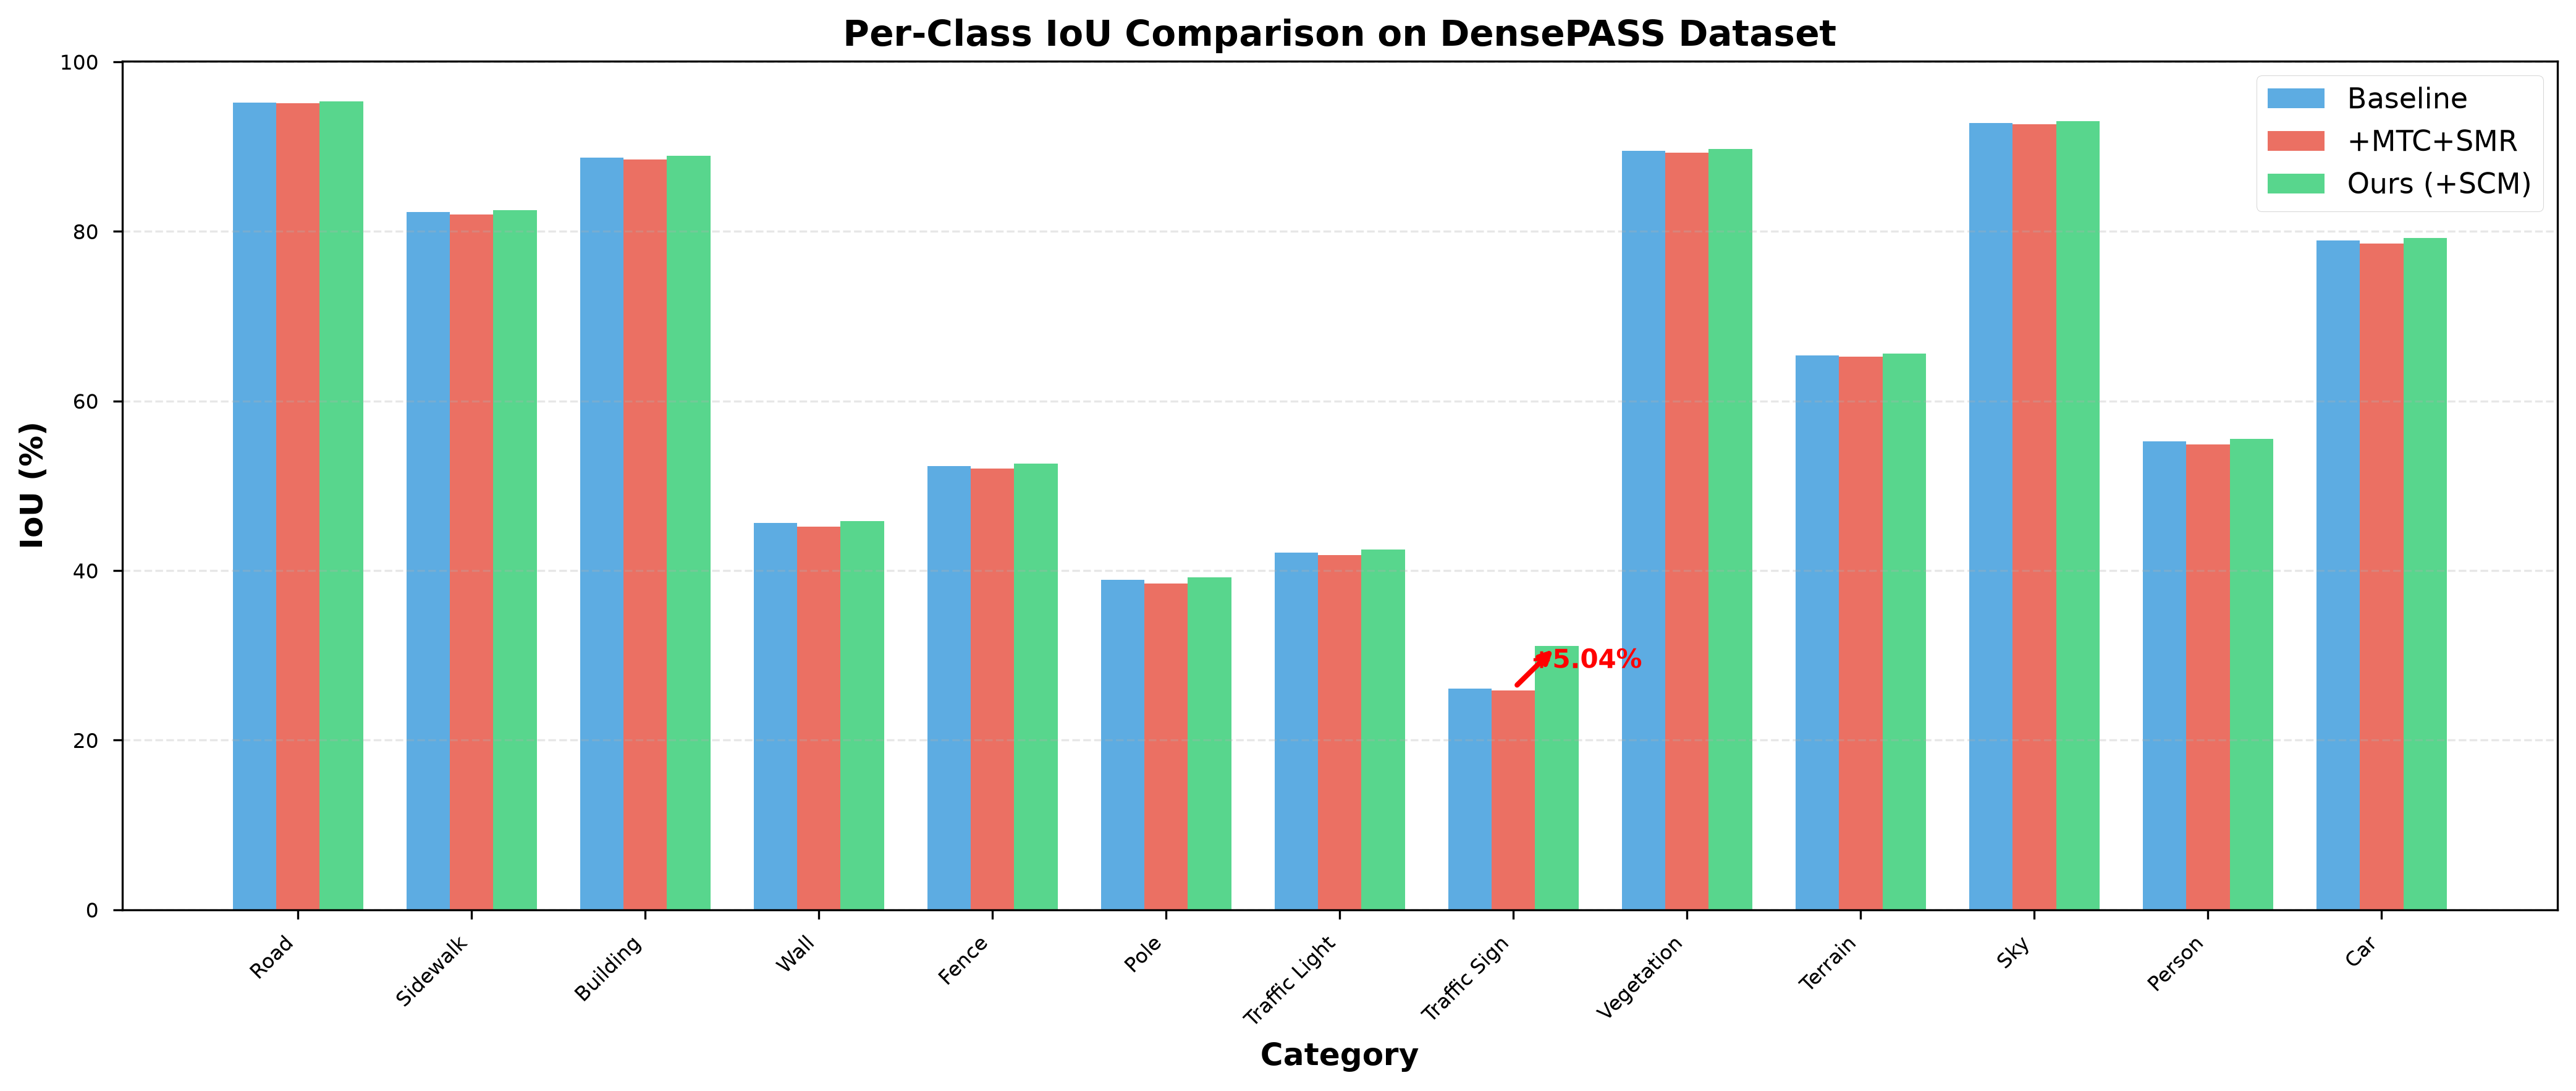
\includegraphics[width=0.95\linewidth]{figures/fig_per_class_iou_comparison.png}
\caption{各类别IoU柱状图对比。交通标志类别（红框标注）提升最显著（+5.04\%），验证了SCM对边界区域的优化效果。}
\label{fig:per_class_comparison}
\end{figure}

\textbf{定性结果对比。}图\ref{fig:qualitative_comparison}展示了不同方法在DensePASS数据集上的定性分割结果。从对比中可以看到，完整方法（MTC+SMR+SCM）在全景图边界区域（左右边缘拼接处）产生了更连续、更准确的分割边界，特别是在交通标志、车辆等小目标类别上表现更好。红框标注处显示，基线方法在边界处产生截断，而我们的方法通过循环记忆恢复了完整的物体上下文。

\begin{figure}[t]
\centering
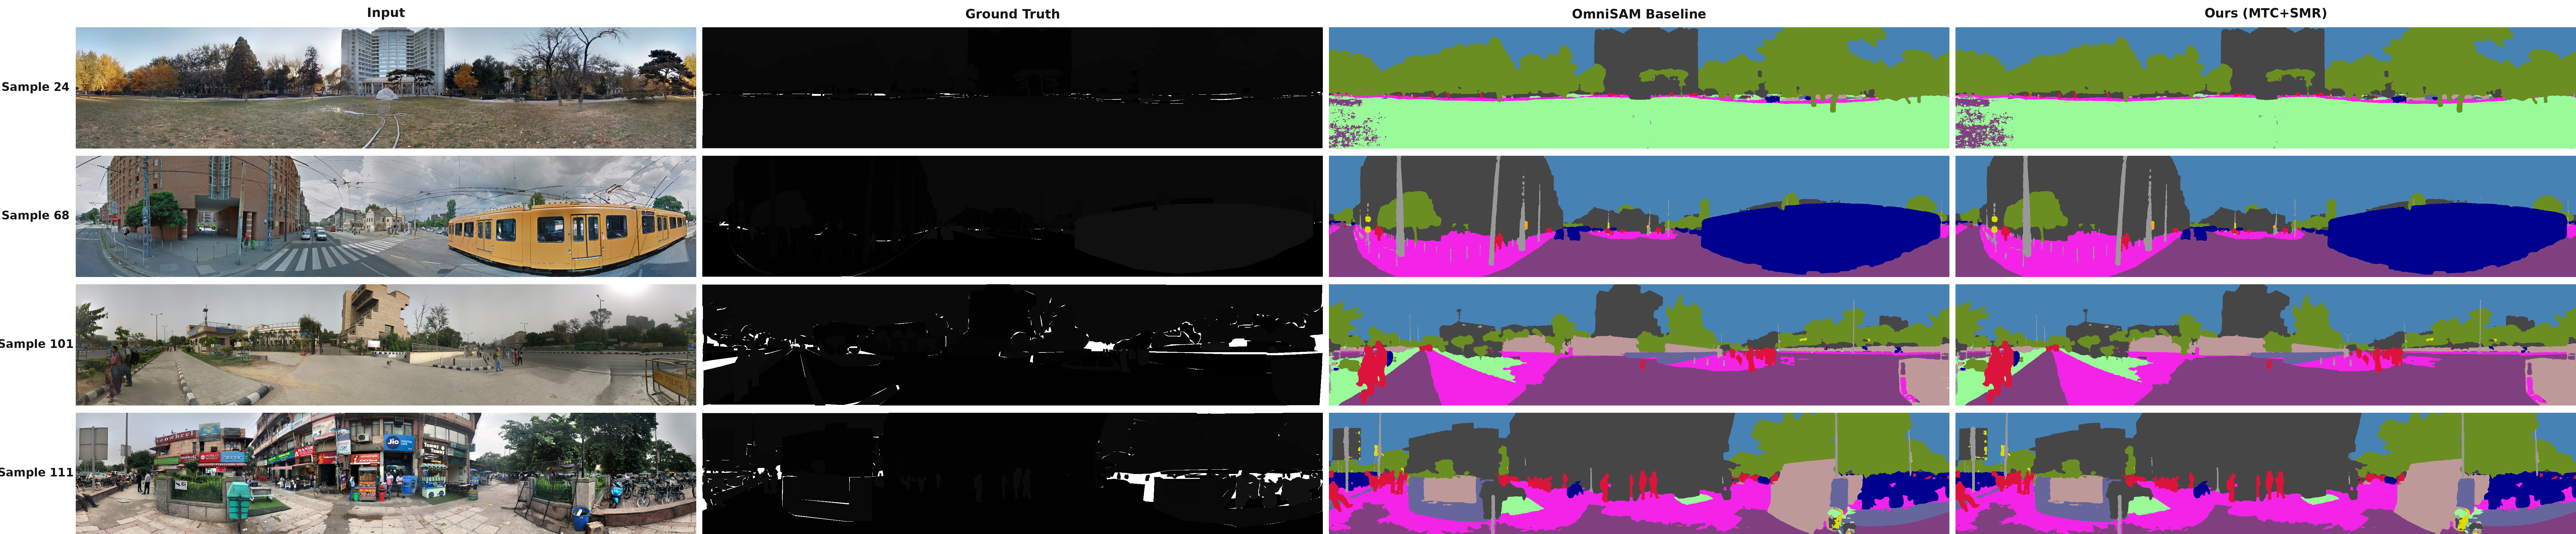
\includegraphics[width=0.95\linewidth]{figures/fig_qualitative_full_protocol.png}
\caption{定性分割结果对比。上：原始全景图像；中：基线方法（OmniSAM）；下：完整方法（MTC+SMR+SCM）。红框标注处显示边界连续性的显著改善。}
\label{fig:qualitative_comparison}
\end{figure}

\subsection{消融实验}

\textbf{Memory模块消融。}表\ref{tab:memory_ablation}采用固定伪标签设置，复用相同伪标签以隔离Memory模块的影响。结果显示，MTC和SMR均能有效降低Memory Tokens和注意力时间，验证了空间压缩和内容选择的互补作用。组合配置将Tokens从32768压至4096，注意力时间降至51.92秒，伴随轻微精度代价（mIoU -0.22\%），体现了效率-精度权衡。

\begin{table}[t]
  \centering
  \small
  \setlength{\tabcolsep}{4pt}
  \renewcommand{\arraystretch}{1.08}
  \caption{固定伪标签消融设置下的 memory-efficient 模块比较。该实验分析 Memory Tokens 与 Memory Attention Time，不作为 full protocol 主结果。}
  \label{tab:memory_ablation}
  \begin{tabular}{lrrrr}
    \toprule
    方法 & Memory Tokens$\downarrow$ & mIoU$\uparrow$ & BFScore$\uparrow$ & Mem. Attn. (s)$\downarrow$ \\
    \midrule
    OmniSAM & 32768 & 60.26 & 39.59 & 117.48 \\
    OmniSAM + Confidence Mask & 32768 & 60.26 & 39.59 & 117.56 \\
    OmniSAM + Confidence Mask + MTC & 8192 & 60.12 & 39.23 & 61.00 \\
    OmniSAM + Confidence Mask + SMR & 16384 & 60.09 & 39.23 & 79.69 \\
    OmniSAM + MTC+SMR & 4096 & 60.02 & 39.23 & 52.38 \\
    OmniSAM + Confidence Mask + MTC+SMR & 4096 & 60.02 & 39.23 & 51.92 \\
    \bottomrule
  \end{tabular}
\end{table}


图\ref{fig:speed_accuracy_tradeoff}展示了不同Memory配置的速度-精度权衡。各配置点展现了不同的效率-精度平衡，MTC+SMR组合在大幅提升效率的同时保持了可接受的精度损失。

\begin{figure}[t]
\centering
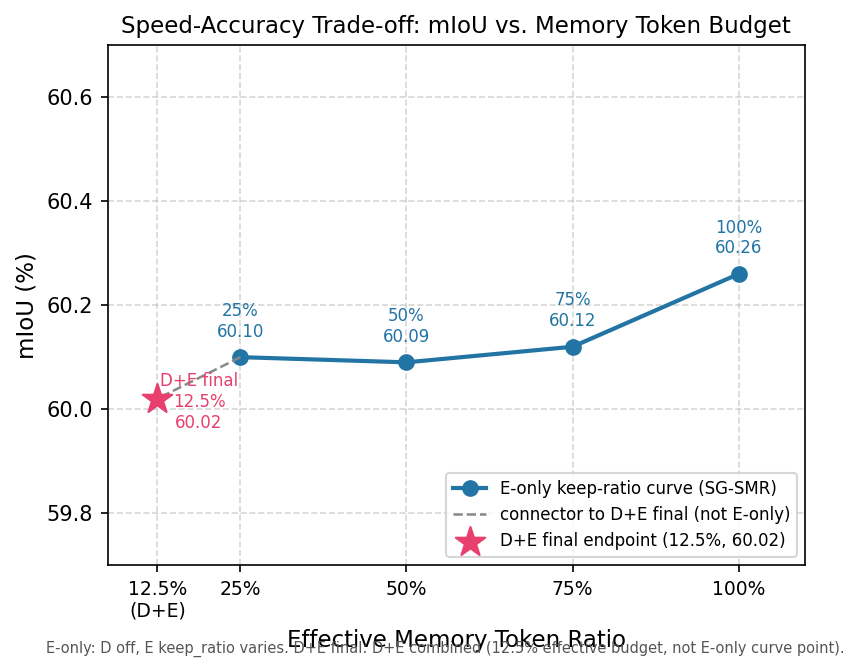
\includegraphics[width=0.78\linewidth]{figures/fig_speed_accuracy_tradeoff_miou.png}
\caption{Memory优化的速度-精度权衡。横轴为训练效率（步时间），纵轴为mIoU。不同配置展示了效率收益与精度变化的关系。}
\label{fig:speed_accuracy_tradeoff}
\end{figure}

\textbf{Token预算消融。}表\ref{tab:token_budget}和图\ref{fig:token_budget_attention_with_scm}显示，注意力时间随Token预算降低而整体下降，而精度仅在较小范围内波动。100\%-25\%区间为仅SMR的曲线（通过调整保留率），12.5\%为MTC+SMR组合端点。加入SCM后（虚线），推理阶段精度显著提升，验证了循环填充对边界区域的优化效果。这表明部分历史记忆可以在不引发性能崩塌的情况下被约简，而SCM能够在推理时有效补偿训练时的精度损失。

\begin{table}[t]
  \centering
  \small
  \setlength{\tabcolsep}{3pt}
  \renewcommand{\arraystretch}{1.08}
  \caption{不同 Memory Token 预算下的精度与效率权衡。结果来自固定伪标签消融设置。}
  \label{tab:token_budget}
  \begin{tabular}{lrrrrr}
    \toprule
    Token 预算 & Tokens$\downarrow$ & mIoU$\uparrow$ & BFScore$\uparrow$ & Step (s)$\downarrow$ & Mem. Attn. (s)$\downarrow$ \\
    \midrule
    100\% & 32768 & 60.26 & 39.59 & 2.4089 & 117.56 \\
    75\% & 24576 & 60.12 & 39.28 & 2.4614 & 98.62 \\
    50\% & 16384 & 60.09 & 39.23 & 2.3798 & 79.69 \\
    25\% & 8192 & 60.10 & 39.29 & 2.2941 & 60.54 \\
    12.5\%$^{\dagger}$ & 4096 & 60.02 & 39.23 & 2.3153 & 51.92 \\
    \bottomrule
  \end{tabular}

  \vspace{0.3em}
  \footnotesize{$^{\dagger}$100\%--25\% 为仅使用稀疏检索的 Token Budget 曲线；12.5\% 为 MTC+SMR 组合端点。}
\end{table}


\begin{figure}[t]
\centering
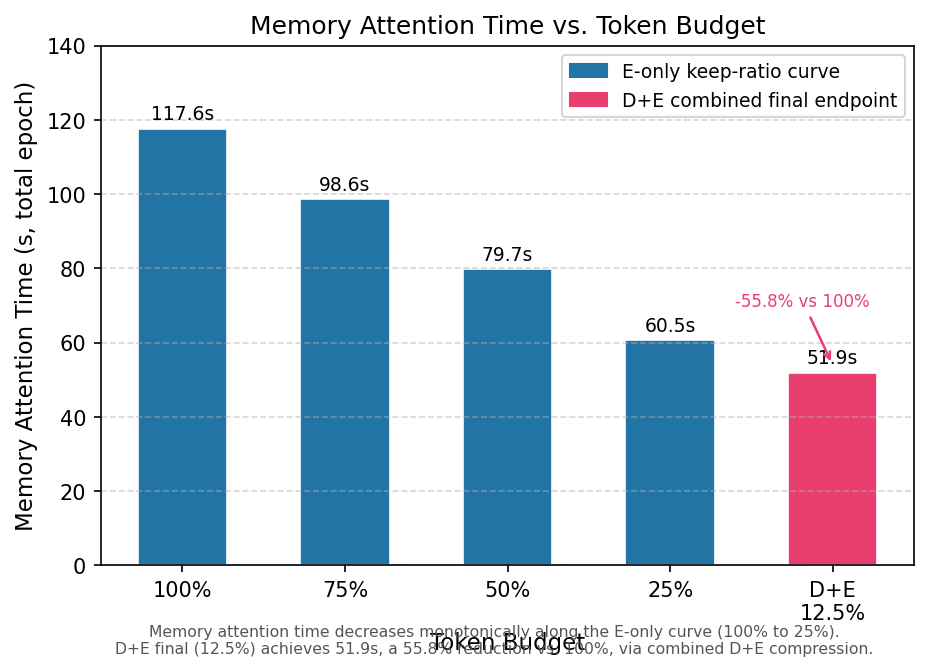
\includegraphics[width=0.78\linewidth]{figures/fig_token_budget_attention_time.png}
\caption{Token预算与注意力时间关系（包含SCM）。100\%-25\%为仅SMR曲线，12.5\%为MTC+SMR组合端点。虚线展示加入SCM后在推理阶段的精度提升，验证了循环填充的有效性。}
\label{fig:token_budget_attention_with_scm}
\end{figure}

\textbf{伪标签优化消融。}表\ref{tab:pseudo_label_ablation}中，类别均衡过滤带来+0.05\% mIoU提升，说明调整类别覆盖可能略微改善监督质量。原型引导门控未进一步改善，可能因为额外过滤减少了有效监督或批次级原型对稀有类别不稳定。PQR作为伪标签可靠性辅助探索，不构成主要贡献。

\begin{table}[t]
  \centering
  \small
  \setlength{\tabcolsep}{4pt}
  \renewcommand{\arraystretch}{1.08}
  \caption{固定伪标签设置下的辅助伪标签质量消融。结果仅用于探索监督可靠性，不构成本文主要性能结论。}
  \label{tab:pseudo_label_ablation}
  \begin{tabular}{lccc}
    \toprule
    方法 & mIoU$\uparrow$ & 相对 R0 & 相对上一配置 \\
    \midrule
    Identity（R0） & 60.02 & -- & -- \\
    类别均衡过滤（R2） & 60.07 & +0.05 & +0.05 \\
    + 原型引导门控（R2+R4） & 60.05 & +0.03 & -0.02 \\
    \bottomrule
  \end{tabular}
\end{table}


综合消融结果表明，MTC+SMR对降低记忆注意力开销的证据最直接，SCM在推理阶段有效补偿了训练时的精度损失，三个模块协同实现了端到端的效率与精度优化。
